Rancangan arsitektur sistem dapat dilihat pada Gambar \ref{fig:arsitektur-sistem}. Sistem ini terdiri dari 3 komponen utama yaitu komponen \textit{data preprocessing}, komponen \textit{data mining}, dan komponen \textit{data integration}. Komponen \textit{data preprocessing} berfungsi untuk membersihkan data dari \textit{noise} dan \textit{outlier}. Komponen \textit{data mining} berfungsi untuk melakukan analisis risiko autentikasi dengan menggunakan metode Random Forest. Komponen \textit{data integration} berfungsi untuk mengintegrasikan sistem dengan sistem FHIR.

\begin{figure}[H]
    \centering
    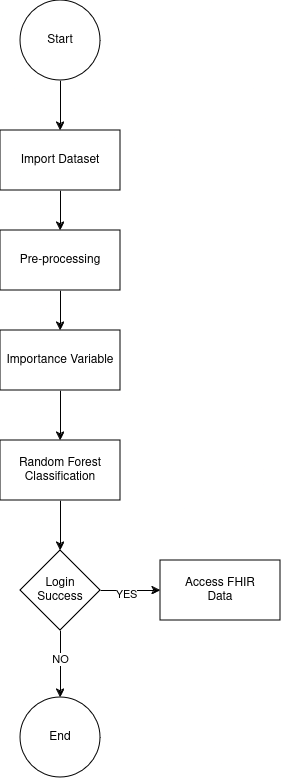
\includegraphics[width=0.5\textwidth]{BAB_TESIS/IMAGES/diagram_kusus.drawio.png}
    \caption{Rancangan Arsitektur Sistem}
    \label{fig:arsitektur-sistem}
\end{figure}

Pada Gambar \ref{fig:arsitektur-sistem}, mengilustrasikan proses sistem yang menggabungkan analisis dataset menggunakan klasifikasi Random Forest dan mekanisme pengendalian akses terhadap data FHIR. Proses dimulai dengan mengimpor dataset yang akan digunakan untuk analisis selanjutnya. Setelah dataset diimpor, langkah berikutnya adalah melakukan pemrosesan awal (pre-processing) guna membersihkan dan mempersiapkan data. Tahapan pre-processing ini meliputi penanganan data yang hilang, normalisasi, dan transformasi data agar siap untuk diterapkan dalam algoritma pembelajaran mesin.

Berikutnya, tahap identifikasi variabel penting dilakukan untuk menentukan fitur yang signifikan dalam dataset. Proses ini mungkin melibatkan analisis statistik atau teknik machine learning untuk memastikan variabel-variabel yang digunakan adalah yang paling relevan untuk klasifikasi. Setelah variabel penting diidentifikasi, data tersebut kemudian diklasifikasikan menggunakan algoritma Random Forest, sebuah metode pembelajaran ensemble yang memanfaatkan beberapa pohon keputusan untuk mencapai hasil yang lebih akurat dan dapat diandalkan.

Langkah selanjutnya adalah verifikasi login pengguna. Sistem akan memeriksa apakah login pengguna berhasil atau tidak. Jika login berhasil, pengguna akan diberikan akses ke data FHIR (Fast Healthcare Interoperability Resources), sebuah standar untuk pertukaran informasi kesehatan elektronik. Jika login gagal, proses akan berakhir tanpa memberikan akses lebih lanjut.

Secara keseluruhan, diagram ini mengintegrasikan metode klasifikasi data dengan langkah verifikasi pengguna untuk mengendalikan akses terhadap data sensitif. Proses ini sangat berguna dalam konteks di mana prediksi berbasis data dan akses berbasis autentikasi sangat penting, seperti dalam analisis data kesehatan atau medis. Implementasi ini memastikan keamanan dan integritas data, sekaligus memberikan hasil analisis yang akurat dan dapat diandalkan.